\chapter{力、夸克與第一批強子多重態}

\section{粒子、場與缺少的第三環}

波是場的組態，因此在目前的討論中，這兩種描述密切相關。量子力學指出，這類波中的能量以離散且不可分割的單位出現。這些單位就是波的量子，而場的量子就是我們所稱的粒子。有了這層關係，我們已經討論過波動方程、作用量原理，以及粒子所具有的廣泛性質：能量、動量、自旋，以及玻色子--費米子之別。費米子不易佔據相同的狀態；玻色子則可以聚集並凝聚於同一狀態。

量子拉格朗日量也記錄了相互作用。場的乘積代表粒子進出頂點的作用。例如，含有場的四次方的項，代表一個四腿相互作用頂點。作用量原理就這樣成為可能粒子過程的精簡清單。

接下來的任務是為粒子命名---不必逐一命名，而是按家族來介紹---並說明每個粒子的特性：它的性質、相互作用，以及在一般物理學中的角色。不過，在列出這份清單之前，概念三角形還缺少一環：
\begin{itemize}
\item 粒子，
\item 以這些粒子為其量子的場，
\item 與涉及這些量子的交換過程相關聯的力。
\end{itemize}

\emph{基本}一詞必須暫且保留。每一種看似合理、用來區分基本粒子與複合粒子的定義，最後都會遇上難以界定的案例；我們稍後會再談這個問題。眼下先假設基本場存在，並稱其量子為基本粒子。如果電場產生電力、重力場產生重力，那麼電子場也必定參與力的作用。只有當力除了場的描述之外，也能以粒子描述，這個三角形才能閉合。

因此，我們會用兩種方式推導力的邏輯。首先從經典場能量出發，再探討將場分解為量子後，同一種相互作用如何呈現。待這座橋梁確立之後，我們才開始列出粒子清單。

\section{經典電動力學中由場能量產生的力}

在空間中放置兩個電荷。求出它們之間的力，一種方法是引用平方反比定律。更能揭示原理的方法，則是探問這些電荷如何影響空間：它們會產生電場，而電場會儲存能量。

將各個電荷與其電場的空間分布分開來看很有用，
\begin{equation}
\mathbf E_i=q_i\widehat{\mathbf E}_i,
\end{equation}
不過，是否保留帽號記法並不影響結果。兩個電荷都存在時，由線性疊加可得
\begin{equation}
\mathbf{E}=\mathbf{E}_1+\mathbf{E}_2.
\end{equation}
除單位制的選擇外，靜電場能量的形式為
\begin{equation}
U_{\text{field}}\propto\int d^3x\,\mathbf{E}^2.
\end{equation}
代入兩個電場之和，可得
\begin{align}
U_{\text{field}}
&\propto\int d^3x\,(\mathbf{E}_1+\mathbf{E}_2)^2 \\
&\propto\int d^3x\,\bigl(\mathbf{E}_1^2+\mathbf{E}_2^2
  +2\mathbf{E}_1\!\cdot\!\mathbf{E}_2\bigr).
\end{align}

前兩項是自能。平移任一電荷時，它的電場也隨之移動，相應的積分不會改變。這部分能量透過\(E=mc^2\)貢獻於孤立帶電粒子的測量質量。如何將這種自能納入測量質量，屬於稍後要談的重整化問題。這些與位置無關的能量都不會對兩個粒子間的力有所貢獻。

交叉項則不同。它不單獨屬於任一粒子，只有兩個電場同時存在時才會出現。如果兩個電荷相距極遠，各自主要分布的電場區域幾乎不重疊；電荷靠近時，重疊情形便會改變。因此，依組態而變的相互作用能與下式成正比
\begin{equation}
U_{\text{int}}(r)\propto q_1q_2\int d^3x\,
\widehat{\mathbf E}_1\!\cdot\!\widehat{\mathbf E}_2.
\end{equation}
兩個點電荷相距\(r\)時，計算此積分可得熟知的關係
\begin{equation}
U_{\text{int}}(r)\propto\frac{q_1q_2}{r}.
\end{equation}
徑向力等於其負梯度，
\begin{equation}
\mathbf F_{12}=-\boldsymbol\nabla_{\mathbf r}U_{\text{int}},
\qquad
|\mathbf F_{12}|\propto\frac{|q_1q_2|}{r^2}.
\end{equation}
\editorialnote{口頭論證直接將交叉項連結到平方反比的庫侖力，沒有停下來說明勢能。這裡明確寫出標準的中間量\(U_{\mathrm{int}}\propto1/r\)，使其梯度可得出上述\(1/r^2\)力。}

力定律現在成了場能量中依賴相對位置的部分之導數。相距甚遠時，兩個物體實際上互不影響。讓它們彼此靠近，它們之間的場便會重新分布；由此引起的能量變化就是相互作用。

然而，既然場可以分解為量子，這個故事就不能到此為止。同一種力也必須能以粒子的語言來描述。

\section{分子交換：兩個質子與一個電子}

回到電動力學之前，先考慮一個較容易想像交換過程的系統：兩個質子和一個電子。交換只是分子力的幾種來源之一，但這個例子能讓交換、能量與力之間的關係具體呈現。這個例子並非用來取代量子電動力學。

若只有一個質子，而另一個位於無窮遠處，電子便可以佔據以第一個質子為中心的類氫基態。它的波函數局域在該力中心附近。

\begin{figure}[h]
\centering
\includegraphics[width=0.72\textwidth]{lecture_01_figure_02.png}

\medskip

\begin{tikzpicture}[scale=0.95]
\draw (-0.2,0) -- (6.4,0);
\fill (1.3,0) circle (2pt);
\draw[smooth] plot coordinates {(0.1,0.15) (0.8,1.15) (1.5,1.75) (2.2,1.1) (3.0,0.35) (3.8,0.12)};
\node at (1.3,-0.35) {$p$};
\node at (2.7,1.55) {$\psi_1(x)$};
\end{tikzpicture}
\caption{局域於一個質子附近的類氫基態波函數。}
\lectureframe{00:14:32}
\end{figure}
\editorialnote{重繪圖中的標籤\(\psi_1(x)\)標示了00:14:30--00:14:32所述的局域分布；這個標籤並非抄自可辨識的板書。}

現在將第二個質子放在相距很遠、但距離有限的位置。由對稱性可知，還有一個能量相同的局域態，這次以右側質子為中心。

\begin{figure}[h]
\centering
\includegraphics[width=0.78\textwidth]{lecture_01_figure_03.png}

\medskip

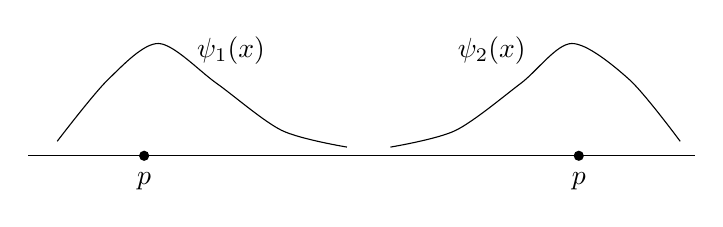
\begin{tikzpicture}[scale=0.92]
\draw (-0.2,0) -- (9.0,0);
\fill (1.4,0) circle (2pt);
\fill (7.4,0) circle (2pt);
\draw[smooth] plot coordinates {(0.2,0.2) (0.9,1.05) (1.6,1.55) (2.4,1.0) (3.3,0.35) (4.2,0.12)};
\draw[smooth] plot coordinates {(4.8,0.12) (5.7,0.35) (6.6,1.0) (7.3,1.55) (8.1,1.05) (8.8,0.2)};
\node at (1.4,-0.35) {$p$};
\node at (7.4,-0.35) {$p$};
\node at (2.6,1.45) {$\psi_1(x)$};
\node at (6.2,1.45) {$\psi_2(x)$};
\end{tikzpicture}
\caption{允許隧穿後，用來形成平衡疊加態的兩個局域分布。}
\lectureframe{00:17:54}
\end{figure}
\editorialnote{標籤\(\psi_1(x)\)和\(\psi_2(x)\)標示了00:17:41--00:17:56所述的兩個分布；這些符號是為了便於辨識而加上的示意標籤。}

兩者相距無窮遠時，這兩個態是簡併的：將電子局域在左側或右側，所需能量相同。距離有限時，一種新的過程便成為可能。電子可以穿隧通過經典上禁阻的區域，從一個中心到達另一個中心。若試圖觀察電子是否沿某條軌跡穿過勢壘，就會擾動這個態；``躍遷''描述的是量子演化，並非一段經典路徑的影片。

在平衡狀態下，電子出現在任一質子附近的機率相同。因此，歸一化因子為\(1/\sqrt2\)，能量較低的平衡態近似為
\begin{equation}
\psi_+(x)\approx \frac{\psi_1(x)+\psi_2(x)}{\sqrt2}.
\end{equation}

近似符號很重要。真正的雙中心波函數並非兩個未受擾動的類氫軌域直接相加；波函數會在重疊區域有所調整。此處需要掌握的是，對稱的平衡態能量低於孤立單中心態的能量。用哈密頓量的語言來說，左側和右側的組態由一個非對角矩陣元素耦合。允許電子處於兩者的相干疊加態，會降低能量。

\section{從能量降低到有效力}

質子相距很遠時，電子所造成的能量貢獻\(E_e(r)\)趨近於原子分離時的值。距離較近時，隧穿和疊加會使此能量降低。完整的雙質子--單電子系統的勢能，還必須包含質子間的直接排斥，
\begin{equation}
V_{\mathrm{tot}}(r)=V_{pp}(r)+E_e(r).
\end{equation}

這讓分子例子與場能量的論證重新連結起來。波函數示意圖和\(E_e(r)\)的定性曲線，是同一項計算的兩種呈現方式；平衡位置由總和\(V_{\mathrm{tot}}(r)\)決定。

\begin{figure}[h]
\centering
\includegraphics[width=0.78\textwidth]{lecture_01_figure_04.png}

\medskip

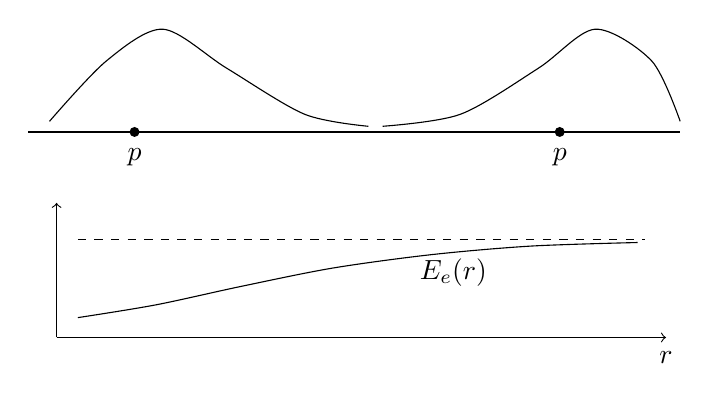
\begin{tikzpicture}[scale=0.9]
\draw (-0.2,3.0) -- (9.0,3.0);
\fill (1.3,3.0) circle (2pt);
\fill (7.3,3.0) circle (2pt);
\draw[smooth] plot coordinates {(0.1,3.15) (0.9,4.0) (1.7,4.45) (2.6,3.9) (3.7,3.25) (4.6,3.08)};
\draw[smooth] plot coordinates {(4.8,3.08) (5.9,3.25) (7.0,3.9) (7.8,4.45) (8.6,4.0) (9.0,3.15)};
\node at (1.3,2.65) {$p$};
\node at (7.3,2.65) {$p$};

\draw[->] (0.2,0.1) -- (0.2,2.0);
\draw[->] (0.2,0.1) -- (8.8,0.1);
\draw[dashed] (0.5,1.48) -- (8.5,1.48);
\draw[smooth] plot coordinates {(0.5,0.38) (1.6,0.56) (2.8,0.82) (4.1,1.08) (5.5,1.27) (6.9,1.39) (8.4,1.44)};
\node at (5.8,1.02) {$E_e(r)$};
\node at (8.8,-0.18) {$r$};
\end{tikzpicture}
\caption{上方是波函數重疊，下方是電子造成的能量。隨著\(r\)增加，能量會逐漸升至原子分離時的漸近值；質子系統的總勢能還必須包含質子間的庫侖排斥。}
\lectureframe{00:20:28}
\end{figure}
\editorialnote{標籤\(E_e(r)\)和\(r\)標示了00:19:12--00:20:38所述的能量曲線與間距；留存的板書畫面無法辨識這些座標軸標籤。}

相應的兩種力可由能量梯度求得，
\begin{equation}
F_{e}(r)=-\frac{dE_e}{dr},
\qquad
F_{\mathrm{tot}}(r)=-\frac{dV_{\mathrm{tot}}}{dr}.
\end{equation}
因此系統會受到作用而趨向總能量較低的狀態。在\(E_e(r)\)隨著質子靠近而降低的區域，交換會帶來吸引作用；是否存在束縛距離，則取決於這種作用與\(V_{pp}(r)\)的競爭。這就是共價鍵背後的基本機制：共享態在能量上較有利，因此電子會被共享。

在經典計算中，電場重疊會改變能量。這裡則是兩個力中心使較低能量的量子態成為可能。兩種機制都會產生力，因為平衡能量取決於組態。

交換的概念可以用世界線示意圖來概括。這不能解讀為觀測到的軌跡；它表示電子與任一質子相關聯的機率振幅。

\begin{figure}[h]
\centering
\begin{tikzpicture}[scale=1.0]
\draw (0,0) -- (0,4.4);
\draw (4.8,0) -- (4.8,4.4);
\draw (0,0.9) .. controls (1.6,1.7) and (3.2,1.7) .. (4.8,2.5);
\draw (4.8,2.9) .. controls (3.2,2.1) and (1.6,2.1) .. (0,3.9);
\node at (0,-0.35) {$p$};
\node at (4.8,-0.35) {$p$};
\node at (2.35,1.55) {$e^-$};
\node at (2.35,2.55) {$e^-$};
\end{tikzpicture}
\caption{兩條質子世界線之間的電子交換；這是量子振幅的示意圖，並非觀察到的路徑。}
\end{figure}

\begin{classroomqa}
\audiencequestion{這種吸引作用能否簡單理解為電子遮蔽或減弱了質子的電荷？\lecturetimestamp{00:23:26}}
\lecturerresponse{不能。電荷減弱不是理解這種效應的恰當圖像。關鍵在於，將兩個局域波函數相加後得到的態，其能量略低於任一局域態單獨存在時的能量。}
\end{classroomqa}

\begin{classroomqa}
\audiencequestion{這就是費曼所說的``光喜歡光''嗎？\lecturetimestamp{00:23:51}}
\lecturerresponse{不是。那句話很可能指的是玻色統計：光子傾向於佔據共同的狀態，而電子則遵守不相容原理。這裡的分子效應是電子在兩個中心之間隧穿。}
\end{classroomqa}

兩個質子仍然會產生靜電排斥。交換作用的作用範圍比庫侖相互作用短，因此必須考慮總勢能，不能只看其中一項。在適當的距離下，分子離子\(\mathrm H_2^+\)仍會形成束縛態；在中性雙電子系統中，長程電荷排斥不存在，共價鍵結也就更為常見。

\begin{classroomqa}
\audiencequestion{把電子放在兩個質子之間，主要作用是減弱它們之間的靜電排斥嗎？\lecturetimestamp{00:24:33}}
\lecturerresponse{這樣做確實會稍微減弱排斥，但這不是主要效應。電子交換作用的作用範圍比庫侖排斥短。在中性雙電子系統中，這種效應最為明顯：原子間沒有長程靜電力，但隧穿仍會產生吸引作用。}
\end{classroomqa}

\begin{classroomqa}
\audiencequestion{帶正電、只有一個電子的分子離子\(\mathrm H_2^+\)真的會形成束縛態嗎？\lecturetimestamp{00:26:06}}
\lecturerresponse{會。在距離足夠近時，交換吸引作用足以克服質子--質子間的庫侖排斥。}
\end{classroomqa}

\begin{classroomqa}
\audiencequestion{雙中心組態會產生第三種力嗎？\lecturetimestamp{00:26:24}}
\lecturerresponse{這裡沒有引入新的基本力。兩個質子的合成勢能中，Schr\"odinger方程的平衡能量與單中心問題不同；改變後的能量對位置的導數，就是有效力。}
\end{classroomqa}

\begin{classroomqa}
\audiencequestion{能量降低是量子糾纏的一個例子嗎？\lecturetimestamp{00:27:06}}
\lecturerresponse{這不是通常所說的雙粒子糾纏，因為只需要一個電子。相關的數學特徵是耦合左右兩個態的非對角哈密頓矩陣元素。}
\end{classroomqa}

\begin{classroomqa}
\audiencequestion{高溫下交換作用會如何變化？\lecturetimestamp{00:27:37}}
\lecturerresponse{在極高溫下，電子會被游離，完全脫離分子。在較低的激發能量下，電子可能佔據較大的軌域，改變波函數重疊，進而改變力。這是依狀態而異的修正，並非新的普遍機制。}
\end{classroomqa}

\section{光子交換與表格中的最初幾項}

庫侖力也能用同樣的交換語言來描述嗎？帶電粒子會與電磁場相互作用，而電磁場的量子就是光子。經典理論中，我們求解電荷周圍的電場；量子場論則將這種相互作用分解為光子的發射與吸收。

物理上的帶電粒子並非只有裸電荷。它的量子態是疊加態，包含裸電子分量、帶有一個光子的電子分量、帶有兩個光子的電子分量，依此類推。用刻意簡化的示意記號表示，
\begin{equation}
\begin{aligned}
\ket{e_{\mathrm{phys}}}
={}&a_0\ket e
+a_1\ket{e+\text{one photon}}
\\
&+a_2\ket{e+\text{two photons}}+\cdots .
\end{aligned}
\end{equation}
這個記號只呈現光子數分量的層級；它沒有指定光子的動量，也沒有試圖完整構造相互作用下的帶電態。
周圍的光子會被發射後再吸收，而不是以自由輻射的形式逃逸。這些光子的效應可以測量，儘管它們的探測方式與自由傳播的光子不同。在附近放置另一個電荷，一個電荷發射的光子便可能被另一個電荷吸收。如此一來，兩個綴飾態的能量便不再等於兩個孤立態的能量總和。

課堂上用兩個雜耍者來比喻，他們各自拋接一組球。相距很遠時，兩人各自獨立拋接；靠得夠近時，其中一人可能接住另一人拋來的球。用費曼圖的語言來說，兩人共享的物體就是交換的光子。這個比喻不是在描繪微觀軌跡，但呈現了為何彼此靠近會使新的過程成為可能。

現在，我們有了兩種不只是背誦庫侖定律的描述方式。經典場論將場相加，再將結果平方；量子場論則對交換量子的振幅求和。就這個意義而言，粒子、場與力彼此一一對應。電子促成分子交換，光子促成電磁交換，而任何可以被交換的粒子，在適當情境下都能對力有所貢獻。因此，熟知的「自然界有四種基本相互作用」是較宏觀層次的分類；從交換的角度來看，每一種可交換的粒子都能產生自身的有效力貢獻。

現在終於可以為粒子命名、列出它們的性質，並說明它們能參與哪些過程。若一次寫出完整的標準模型，只會變成冗長的記憶測驗。因此我們會把粒子分成若干小組；同組成員之間的關係簡單明確，並逐組了解它們能參與哪些過程。

完整的粒子清單十分繁複，因為我們還不明白為什麼偏偏存在這些粒子，而不是其他可以想像的粒子。數學自洽性提供了一些關係：某種模式中的幾個成員一旦存在，或許就必須有另一個成員才能補全模式。這些關係能減少獨立事實的數目，但幅度有限。許多粒子種類和參數仍未獲得解釋。若要了解後續實驗試圖發現什麼，就必須理解這個尚未完成的架構。

\begin{figure}[h]
\centering
\includegraphics[width=0.7\textwidth]{lecture_01_figure_05.png}
\caption{粒子表的第一項以\(\gamma\)標示光子，並以向量勢\(A\)標示其場。}
\lectureframe{00:39:11}
\end{figure}

第一個場--量子對應關係為
\begin{equation}
\gamma \leftrightarrow A.
\end{equation}
此處\(A\)表示電磁向量勢。光子是自旋為一的玻色子，電荷、重子數與靜止質量皆為零。電子場通常記作\(\psi_e\)；其產生算符與湮滅算符作用於電子態和正電子態。

表格列出名稱、粒子符號、場、玻色子或費米子類型、電荷\(Q\)、重子數\(B\)以及質量：

\begin{table}[h]
\centering
\resizebox{\linewidth}{!}{%
\begin{tabular}{lllllll}
名稱&符號&場&類型&\(Q\)&\(B\)&質量\\
光子&\(\gamma\)&\(A\)&玻色子&\(0\)&\(0\)&\(0\)\\
電子&\(e^-\)&\(\psi_e\)&費米子&\(-1\)&\(0\)&\(0.51\,\mathrm{MeV}\)\\
正電子&\(e^+\)&\(\psi_e\)&費米子&\(+1\)&\(0\)&\(0.51\,\mathrm{MeV}\)
\end{tabular}
}%
\caption{粒子清單開頭的光子與電子--正電子項目。}
\end{table}

電子與正電子彼此互為反粒子。將帶負電的態``稱為粒子''只是一種約定。我們以電子電荷量值為單位測量電荷，因此
\begin{equation}
Q(e^-)=-1,\qquad Q(e^+)=+1.
\end{equation}
使用\(E=mc^2\)，質量可以用能量單位表示。一電子伏特是電荷\(e\)通過一伏特的電位差所獲得的能量，
\begin{equation}
1\,\mathrm{eV}=e\,(1\,\mathrm V).
\end{equation}
這個單位源自原子物理中的自然尺度：氫原子的游離能約為\(13.5\,\mathrm{eV}\)。粒子質量則需要用數百萬或數十億電子伏特表示。電子質量為
\begin{equation}
m_e c^2 \approx 0.511\,\mathrm{MeV}.
\end{equation}

\begin{classroomqa}
\audiencequestion{電子質量是否恰好是半個MeV？\lecturetimestamp{00:44:02}}
\lecturerresponse{不是。方便使用的約略值\(0.51\,\mathrm{MeV}\)並非由任何原理固定為精確的一半；它是實驗測得的參數。}
\end{classroomqa}

基本的QED過程包含一條帶電費米子線進入頂點、一條離開頂點，並接上一條光子線。重新排列或交叉這些外腿後，同一個頂點可以描述光子的發射、吸收，或正電子過程。以此處使用的非協變示意記法表示，相互作用項包含
\begin{equation}
\mathcal{L}_{\mathrm{int}}\sim e\,\psi_e^\dagger \psi_e A.
\end{equation}
將場展開為產生與湮滅算符後，會得到一些項，分別移除一個入射電子、產生一個出射電子，以及產生或湮滅一個光子。耦合常數\(e\)在頂點提供一個因子。因此，電子散射或加速時發射光子的情況有
\begin{equation}
\mathcal{A}_{\mathrm{vertex}}\propto e,
\qquad
P_{\mathrm{emission}}\propto e^2.
\end{equation}
X光管中，電子撞擊靶材，就是光子發射機率會發揮作用的實際例子。同一個頂點反覆組合，就會產生量子電動力學中的各種過程，包括被解釋為電荷間作用力的能量位移。

因此，畫出頂點示意圖很有用。

\begin{figure}[h]
\centering
\begin{tikzpicture}[scale=1.0]
\fill (0,0) circle (1.5pt);
\draw (-1.6,-1.2) -- (0,0) -- (1.6,-1.2);
\draw (0,0) -- (0,1.8);
\node at (-1.8,-1.4) {$e^-$};
\node at (1.8,-1.4) {$e^-$};
\node at (0.35,1.95) {$\gamma$};
\end{tikzpicture}
\caption{基本QED頂點的拓撲示意圖：一條帶電費米子線進入頂點，一條離開頂點，並接上一個光子。此處將光子腿畫成直線，只是簡化的繪圖慣例。}
\end{figure}

兩個這樣的頂點相連，就形成力的交換貢獻：

\begin{figure}[h]
\centering
\begin{tikzpicture}[scale=1.0]
\draw (0,0) -- (0,4.0);
\draw (4.8,0) -- (4.8,4.0);
\draw (0,2.0) -- (4.8,2.0);
\node at (0,-0.35) {$e^-$};
\node at (4.8,-0.35) {$e^-$};
\node at (2.4,2.3) {$\gamma$};
\end{tikzpicture}
\caption{光子交換的拓撲示意圖，呈現庫侖相互作用的量子場論描述。}
\end{figure}

粒子--場--力的三角形已經閉合，我們可以繼續列出粒子清單。

\section{夸克、重子數與家族之謎}

如果這份清單是在1960年前後編寫，質子和中子很可能會排在電子和光子之後。現代粒子物理學則先介紹夸克。在簡化的組成粒子圖像中，質子和中子是較大的複合體，由更小的夸克自由度構成。\emph{複合}的確切含義仍有待探討，但組成粒子的觀點已極為有用。

所有夸克都是費米子，並帶有重子數。重子數是核物理中為計算核子數而引入的量。\emph{核子}特指質子或中子。\emph{重子}則是範圍更廣的類別，包含核子以及稍後會介紹的類似重粒子。質子與中子的重子數各為一，
\begin{equation}
B(p)=B(n)=1,
\qquad
B(\bar p)=B(\bar n)=-1.
\end{equation}
對原子核而言，重子數恰好等於質量數\(A=Z+N\)，也就是質子數加上中子數。以原子質量單位測得的原子質量數值，只是近似等於\(A\)。在{\proseunicodefont β}衰變等過程中，質子可以轉變為中子，中子也可以轉變為質子，但核子總數不變。例如，
\begin{equation}
n\longrightarrow p+e^-+\bar\nu_e
\end{equation}
會分別改變質子數與中子數，同時維持兩者總和不變。

\begin{classroomqa}
\audiencequestion{同位素是否與質子數加中子數守恆相矛盾？\lecturetimestamp{00:52:03}}
\lecturerresponse{不同同位素的中子數確實不同，而{\proseunicodefont β}衰變能使中子與質子互換。在一般核過程中，守恆的是總重子數，而非質子數或中子數各自守恆。}
\end{classroomqa}

這種正規化方式是約定俗成的。我們原本也可以將質子的重子數定為\(2\)、\(7\)或\(\pi\)，只要所有複合粒子的重子數都按相同比例調整即可。一旦將質子的重子數定為\(B=1\)，並假設它由三個夸克組成，每個夸克就必須帶有
\begin{equation}
B(q)=\frac13,
\qquad
B(\bar q)=-\frac13.
\end{equation}
因此，這個分數值是歷史上的結果：先將複合核子的重子數正規化，再據此設定夸克的重子數。

\begin{classroomqa}
\audiencequestion{夸克數守恆嗎？\lecturetimestamp{00:54:23}}
\lecturerresponse{夸克--反夸克對可以產生或湮滅，因此夸克總數並不守恆。與重子數相對應的量是夸克數減去反夸克數，再除以三。實驗上，這個量在極高精度下守恆，但此處不將其假設為絕對定律。}
\end{classroomqa}

例如，假設有一種守恆電荷的衰變過程
\begin{equation}
p\longrightarrow e^++\gamma
\end{equation}
這會使重子數為一的初態轉變成重子數為零的末態。這只是用來說明計數方式的例子，並非提出一種衰變模型。目前尚未觀察到任何違反重子數守恆的過程。此處引用的粗略下限，表示質子壽命至少在\(10^{33}\)--\(10^{34}\)年的量級。沒有人會等上那麼久來觀察單一質子；實際做法是以龐大的質子樣本觀察一段可行的時間，藉由增加樣本數來補足觀察時間。儘管如此，當時普遍預期質子會衰變，而目前討論的數學並未提供絕對的禁止。因此，重子數是否嚴格守恆仍是未解的實驗問題：尚未觀察到違反現象、受到嚴格限制，但尚未遭到排除。

\begin{classroomqa}
\audiencequestion{質子--反質子湮滅會違反重子數守恆嗎？\lecturetimestamp{00:56:17}}
\lecturerresponse{不會。初態的重子數為\(1+(-1)=0\)，因此湮滅為重子數為零的末態仍符合守恆。孤立質子衰變為非重子產物才會違反重子數守恆。}
\end{classroomqa}

夸克有六種味，
\begin{equation}
u,\ d,\ s,\ c,\ b,\ t,
\end{equation}
分別稱為上、下、奇異、粲、底和頂。上夸克沒有任何朝上的特性，奇異夸克也不比其他夸克更奇異；這些名稱反映的是歷史，而非物理原理。場的記號並不完全一致：有時使用\(q\)、\(Q\)、\(\psi_q\)，也有人直接用味的字母\(u,d,s,c,b,t\)同時表示場及其量子。

\begin{classroomqa}
\audiencequestion{底夸克和頂夸克，就是以前稱為美夸克和真夸克的粒子嗎？\lecturetimestamp{00:58:35}}
\lecturerresponse{是的。較簡潔的名稱「底」和「頂」後來成為標準用法。名稱的沿革不涉及任何動力學內容。}
\end{classroomqa}

它們的電荷模式以三對重複出現：
\begin{equation}
\begin{aligned}
Q(u)=Q(c)=Q(t)&=+\frac23,
\\
Q(d)=Q(s)=Q(b)&=-\frac13.
\end{aligned}
\end{equation}
反夸克帶有相反的電荷和重子數。從未觀察到孤立的分數電荷，因為夸克不會以自由的漸近粒子形式出現；觀察到的強子都帶有整數電荷。

\((d,u)\)、\((s,c)\)和\((b,t)\)是三個家族，它們重複出現相同的電荷模式。六種夸克的重子數皆為\(B=1/3\)。

\begin{classroomqa}
\audiencequestion{較重的夸克也帶有重子數\(1/3\)嗎？\lecturetimestamp{01:02:02}}
\lecturerresponse{是。每種夸克的重子數都是\(1/3\)。}
\end{classroomqa}

質量則沒有呈現類似的重複模式。以下是有用的數量級估值：
\begin{align}
m_u &\sim 5\,\mathrm{MeV},
&
m_d &\sim 10\,\mathrm{MeV},
\\
m_s &\sim 100\,\mathrm{MeV},
&
m_c &\sim 10^3\,\mathrm{MeV},
\\
m_b &\sim 5\,\mathrm{GeV},
&
m_t &\sim 170\,\mathrm{GeV}.
\end{align}
這裡\(1\,\mathrm{GeV}=10^3\,\mathrm{MeV}\)；改用不同單位，底夸克和頂夸克的數值才容易閱讀。下夸克的估計質量遠高於電子的\(0.511\,\mathrm{MeV}\)，但遠低於質子約\(940\,\mathrm{MeV}\)的質量；前者約為\(1{,}800\)個電子質量。事實上，把兩個輕上夸克和一個下夸克的質量相加，仍遠不足以達到質子質量；強子的其餘能量最終也必須納入計算。

\editorialnote{口頭比較時曾說，一個\(10\,\mathrm{MeV}\)的下夸克約有五十個電子那麼重。依照這裡列出的粗略數值，\(10/0.511\approx20\)；質量層級的判斷正確，但「五十倍」是算術上的失誤。}

即使是同一對夸克之內，質量排序也不相同：下夸克比上夸克重，而粲夸克則遠比奇夸克重。頂夸克的質量是上夸克的數萬倍，儘管兩者的電荷和相互作用模式十分相似。

這裡其實有兩個謎題。我們不明白為什麼夸克家族至少存在一代，儘管第一代至少提供了質子、中子和普通物質所需的上夸克與下夸克。我們也不明白自然界為什麼在第二代和第三代重複這種模式，也不明白為什麼這些重複出現的粒子，其質量分布跨越如此多個數量級。雖然已有一些想法，但目前還沒有公認的解釋能計算出這種模式。

\begin{classroomqa}
\audiencequestion{如果頂夸克質量沒有根本性的解釋，那麼在直接發現它之前，人們是如何預估其近似值的？\lecturetimestamp{01:05:53}}
\lecturerresponse{這項估計並非從更深層的原理推導出質量。做法是假設一個候選質量，計算虛頂夸克會如何影響已精確測量的過程，再判斷哪個質量值與觀測結果相符。間接敏感度可以用來限定一個參數，卻不能解釋自然界為什麼選擇這個值。}
\end{classroomqa}

\begin{classroomqa}
\audiencequestion{如果自由夸克無法被單獨分離出來，那麼夸克是在什麼意義上被探測到的？\lecturetimestamp{01:08:04}}
\lecturerresponse{夸克造成的證據可以被探測到：夸克的產生會留下具有特徵的能量、方向和粒子噴注，而虛夸克也會影響其他可觀測量。無法製備的是一個與所有強子伴粒子分離、並能作為孤立漸近粒子加以研究的單獨夸克。}
\end{classroomqa}

\begin{classroomqa}
\audiencequestion{電荷\(-1/3\)和\(+2/3\)的模式是從理論推導出來的，還是只是一種記帳方式？\lecturetimestamp{01:09:02}}
\lecturerresponse{這種模式有一部分是數學一致性所要求的，但並非全部。在這個階段，我們先把這些電荷記錄為已知事實；要等標準模型的其他部分建立之後，才會討論一致性條件。}
\end{classroomqa}

只有\(u\)和\(d\)夸克在普通物質中具有可觀的豐度。較重的味會衰變成較輕的狀態。因此，上夸克和下夸克的相對豐度，主要取決於宇宙和原子核中的質子與中子數量，以及它們的組成。

\begin{classroomqa}
\audiencequestion{宇宙中六種夸克味的相對豐度由什麼決定？\lecturetimestamp{01:09:49}}
\lecturerresponse{穩定物質基本上只含有上夸克和下夸克；較重的味會衰變。自由中子會衰變，而質子在已觀測的時間尺度內是穩定的；不過，束縛在原子核中的中子仍然很多。在這個層次上，計算上夸克和下夸克的數量，歸根究柢就是計算質子和中子的數量。}
\end{classroomqa}

\section{從夸克到強子：核子、奇異重子與介子}

知道夸克的電荷後，就能重新組合出熟悉的強子。中子和質子各含有三個價夸克：
\begin{equation}
n=ddu,
\qquad
p=uud.
\end{equation}
它們的電荷一算便知：
\begin{align}
Q(n) &= Q(d)+Q(d)+Q(u)
= -\frac13-\frac13+\frac23
=0,\\
Q(p) &= Q(u)+Q(u)+Q(d)
= \frac23+\frac23-\frac13
=1.
\end{align}

暫且把光子放在一旁。關掉電磁作用後，質子和中子看起來幾乎是同一種粒子，只是\(u\)和\(d\)互換了位置。這種近似對稱並不完全，因為這兩種夸克的質量並不完全相同。要等到介紹相應的輕介子之後，我們才會為這種對稱性命名並進一步討論。

由於\(m_d>m_u\)，含有兩個下夸克的中子，其夸克質量貢獻應該較大。電磁自能的影響則相反：帶電的質子具有電場能量，而中子沒有淨電荷。自然界中的結果是中子略重。在這個粗略近似下，
\begin{align}
m_pc^2&\approx940\,\mathrm{MeV},\\
m_nc^2&\approx940\,\mathrm{MeV},\\
(m_n-m_p)c^2&\approx1.4\,\mathrm{MeV}.
\end{align}

\begin{classroomqa}
\audiencequestion{質子和中子的質量是多少？\lecturetimestamp{01:15:35}}
\lecturerresponse{在這個粗略的近似下，兩者的質量都接近\(940\,\mathrm{MeV}\)，差約\(1.4\,\mathrm{MeV}\)。}
\end{classroomqa}

這微小的質量差仍足以讓自由中子衰變。扣除電子的靜止能量後，剩餘能量可以轉化為\(n\to p+e^-+\bar\nu_e\)的動能。

同樣的組分邏輯也能組成奇異重子。由於\(s\)和\(d\)的電荷相同，可以用奇夸克取代下夸克，而不改變電荷組合：
\begin{equation}
uds,\qquad uss,\qquad uus.
\end{equation}
因此在上述例子中，\(uds\)和\(uss\)是中性的，而\(uus\)的電荷為\(+1\)。這類狀態的名稱包括\(\Lambda\)和\(\Xi\)；現階段不必詳細說明這些名稱分別指什麼。以\(s\)取代\(d\)，在定性上類似於在相關原子核中以一種核子取代另一種：大部分束縛模式維持不變，但組分的改變會使質量有所變化。這些狀態比普通核子重，並會衰變成較輕的重子，以及攜帶能量和其他守恆量子數所需的額外粒子。

\begin{classroomqa}
\audiencequestion{奇異重子衰變時會產生什麼？\lecturetimestamp{01:19:02}}
\lecturerresponse{會產生質子或中子等較輕的重子，但它不可能是唯一產物：多出的能量和守恆量子數要求還要有其他粒子。詳細的衰變規則留待之後討論。}
\end{classroomqa}

詳細的組分替換規則比這份初步清單複雜得多，不過有一種替換方式是確定可行的：以具有相同電荷的另一種味取代原來的味。在這種粗略的組分估算下，以奇夸克取代下夸克，質量約增加\(90\,\mathrm{MeV}\)。因此，這些重子比質子和中子稍重。它們能衰變成較輕的核子，所以在普通物質和我們周遭的宇宙中並不常見。

\begin{classroomqa}
\audiencequestion{每個重子是否都有一個反重子，只要把其中每個夸克換成對應的反夸克即可？\lecturetimestamp{01:20:33}}
\lecturerresponse{是。把每個組分換成其反粒子，就會得到反質子、反中子或相應的反奇異重子，所有可加性電荷都會反號。}
\end{classroomqa}

\begin{classroomqa}
\audiencequestion{如果改用底夸克取代奇夸克，結果會如何？\lecturetimestamp{01:21:00}}
\lecturerresponse{結果會是底重子。``奇異重子''特指含有\(s\)夸克的重子；「奇異」這個形容詞指的是夸克味，而不是一般意義上的陌生程度。}
\end{classroomqa}

形容詞\emph{奇異}源自這段歷史：當時物理學家已熟悉質子和中子，於是新發現的粒子相較之下顯得出乎意料。了解夸克味的結構後，就會知道這些粒子的存在並不比其他夸克複合粒子更奇特。

組分質量凸顯了一個重要的提醒。把兩個上夸克和一個下夸克的質量相加，只有幾十 MeV，遠不及質子約\(940\,\mathrm{MeV}\)的質量。這種簡單加總漏掉了相當重要的部分。質子和中子也含有膠子，而膠子會攜帶能量。對相對論性束縛系統而言，複合粒子的質量並不能藉由簡單相加各組分所列的質量來求得。

\begin{classroomqa}
\audiencequestion{質子和中子看似缺少的質量來自哪裡？膠子有質量嗎？\lecturetimestamp{01:21:26}}
\lecturerresponse{在這種記帳方式中，膠子不帶重子數，但會攜帶能量。正因為膠子帶有能量，質子或中子的質量才不等於所列輕夸克質量的總和。}
\end{classroomqa}

\begin{classroomqa}
\audiencequestion{這項缺少的貢獻是一種束縛能嗎？\lecturetimestamp{01:22:03}}
\lecturerresponse{是，可以把它稱為一種束縛能。需要留意的是，相對論性複合粒子的質量，並不像把組分質量參數相加所暗示的那樣簡單相加。}
\end{classroomqa}

\begin{classroomqa}
\audiencequestion{複合質子能否用場的語言描述，就像用粒子的語言描述一樣？\lecturetimestamp{01:22:45}}
\lecturerresponse{可以，但困難得多。就此處要建立的組分記帳方式而言，使用粒子的語言遠比直接組合空間上延展的場來得清楚。}
\end{classroomqa}

\begin{classroomqa}
\audiencequestion{相對於分離的組分，普通束縛能是負的。為什麼核子的動力學貢獻卻是很大的正能量？\lecturetimestamp{01:23:32}}
\lecturerresponse{通常對負束縛能的直觀理解不適用於這個情況。這個問題要到後續討論強相互作用時才能解釋，因此目前先擱置。}
\end{classroomqa}

為什麼三個夸克會形成重子，而兩個夸克卻不會形成孤立的雙夸克強子？在夸克理論發展初期，這確實是個謎題。一種可能的回答是：觀測到的束縛組合，其電荷必須是電子電荷的整數倍。單憑這點聽起來像是循環論證：它描述了這種模式，卻沒有解釋原因。儘管如此，這條規則後來證明指向了正確方向；要理解其更深層的起源，則必須先進一步了解強相互作用。現階段，我們明確把它當作一條工作規則：三個夸克可以組成重子，夸克與反夸克可以組成介子，而觀測到的複合粒子電荷都是整數。

由三個相同輕味夸克組成的重子也存在，不過可以等介紹介子之後再談它們的細節。

介子是由\(q\bar q\)組成的複合粒子。它們的重子數為零：
\begin{equation}
B(q\bar q)=\frac13-\frac13=0.
\end{equation}
最輕的例子由\(u\)和\(d\)組成。這些夸克味比其他味輕得多，在普通物質中穩定或衰變得相對慢，在自然界中的豐度也很高。由於產生所需的能量閾值較低，碰撞也較容易產生它們，而不是較重味的夸克複合粒子。基於這些原因，實驗上最早觀測到的介子都是由輕夸克組成，從它們開始介紹最為自然。

自然的味基底為
\begin{equation}
\ket{\bar u d},\qquad \ket{u\bar d},\qquad \ket{\bar u u},\qquad \ket{\bar d d}.
\end{equation}
這次初步計數不施加其他限制：保留四種輕夸克--反夸克配對，再計算各配對的電荷。

帶電態很容易確定。由於\(Q(\bar u)=-2/3\)和\(Q(d)=-1/3\)，
\begin{align}
Q(\bar u d)&=-\frac23-\frac13=-1,
&
\ket{\pi^-}&=\ket{\bar u d}.
\end{align}
把每個組分換成其反粒子，就會得到\(u\bar d\)；因此第二個態是第一個態的反粒子：
\begin{align}
Q(u\bar d)&=+\frac23+\frac13=+1,
&
\ket{\pi^+}&=\ket{u\bar d}.
\end{align}

同味夸克與反夸克組成的態是中性的，但兩種配對各自都沒有獨立的粒子名稱。量子力學允許將它們疊加，形成兩個歸一化且彼此正交的組合：
\begin{align}
\ket{\pi^0} &\approx \frac{\ket{\bar u u}-\ket{\bar d d}}{\sqrt2},\\
\ket{\eta} &\approx \frac{\ket{\bar u u}+\ket{\bar d d}}{\sqrt2}.
\end{align}

\begin{figure}[h]
\centering
\includegraphics[width=0.82\textwidth]{lecture_01_figure_06.png}
\caption{對稱的中性組合被認定為\(\eta\)介子，反對稱組合則歸入{\proseunicodefont π}介子三重態。}
\lectureframe{01:32:35}
\end{figure}

每個中性態都是由夸克--反夸克對構成的糾纏態；糾纏所涉及的不是普通自旋，而是\emph{上味}和\emph{下味}。若在數學上把上味和下味視為類似自旋二分之一變數的兩個方向，那麼上式中的和與差，便扮演著類似熟悉的兩自旋疊加態的角色。這種自旋的內部類比稱為\emph{同位旋}。沒有任何東西真的在空間中朝上或朝下；這兩個方向分別代表\(u\)和\(d\)味。

三種{\proseunicodefont π}介子\(\pi^+\)、\(\pi^0\)和\(\pi^-\)構成同位旋三重態。它們的質量幾乎相同；如果上夸克和下夸克的質量完全相等，三者的質量就會更加接近。與它們正交的中性態稱為\(\eta\)。

\(\eta\)的質量遠大於{\proseunicodefont π}介子：
\begin{equation}
m_\pi \approx 140\,\mathrm{MeV},
\qquad
m_\eta \approx 500\,\mathrm{MeV}.
\end{equation}
\(\eta\)為什麼與其他粒子如此不同，長期以來一直是個謎。如今這個問題已有了解釋，但數學上相當抽象，因此這裡不予推導。

\begin{classroomqa}
\audiencequestion{這些介子的壽命相對較長嗎？\lecturetimestamp{01:33:59}}
\lecturerresponse{若與許多透過強作用衰變的粒子相比，是的。在這裡討論的衰變通道中，它們不會透過強作用衰變；弱作用和電磁作用造成的衰變較慢，因此它們的壽命較長。}
\end{classroomqa}

\begin{classroomqa}
\audiencequestion{中性態\(\bar u u\)和\(\bar d d\)各自有自己的名稱嗎？\lecturetimestamp{01:34:29}}
\lecturerresponse{沒有。具有名稱的是由兩者的和與差形成的線性組合；這些組合具有確定值。}
\end{classroomqa}

\begin{classroomqa}
\audiencequestion{這種中性態疊加與中微子振盪相似嗎？\lecturetimestamp{01:34:44}}
\lecturerresponse{兩者在涉及量子疊加這一點上相似，但相似之處僅止於此。這裡的問題更接近兩個自旋二分之一組分的自旋組合，以及這類態的兩種糾纏方式。這部分留待下一講討論。}
\end{classroomqa}

引入奇夸克後，以\(s\)或\(\bar s\)取代\(d\)或\(\bar d\)，就能得到四種奇異介子或\(K\)介子的味態：
\begin{equation}
\bar u s,\qquad u\bar s,\qquad \bar d s,\qquad d\bar s.
\end{equation}
它們的電荷分別為：
\begin{align}
Q(\bar u s) &=-1,
&
Q(u\bar s) &=+1,
\\
Q(\bar d s) &=0,
&
Q(d\bar s) &=0.
\end{align}
因此，K介子有兩種帶電態和兩種中性態。

初步計數得到三種{\proseunicodefont π}介子、四種K介子和一種\(\eta\)，合計八種態。但這份清單還沒有納入\(\ket{s\bar s}\)配對。因此，三種夸克味與三種反夸克味所能構成的完整基本組合數為
\begin{equation}
3\times3=9.
\end{equation}
缺少的\(s\bar s\)態補足了九種夸克--反夸克味組合。